\myparagraph{Abstract} 


\myparagraph{Publication} This study has been published in \fullcite{Gelmetti2017}.

\section{Interpretation of \gls{jsc} and \gls{ff} from Current-Voltage Sweeps}

\section{Interpretation of Transient PhotoCurrent}\label{interpretation_tpc}

\section{Interpretation of Differential Capacitance}\label{interpretation_dc}

A common commercial capacitor has a capacitance which is a constant, as can be seen in Fig.~\ref{fig:cap_voltage_dependence_commercial}

\begin{figure}%[!hbtp]%
	\centering
	\begin{subfigure}[t]{0.45\textwidth}
		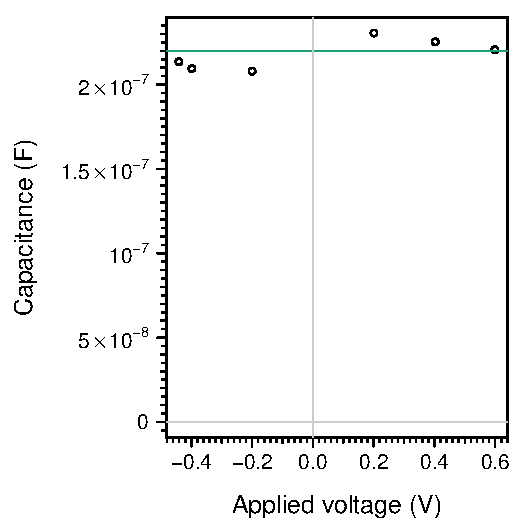
\includegraphics[width=1\textwidth]{cap_voltage_dependence/reference220nF/reference220nF.pdf}
		\subcaption{Commercial \SI{220}{\nano\F} capacitor.}\label{fig:cap_voltage_dependence_commercial}
	\end{subfigure}
	\qquad
	\begin{subfigure}[t]{0.45\textwidth}
		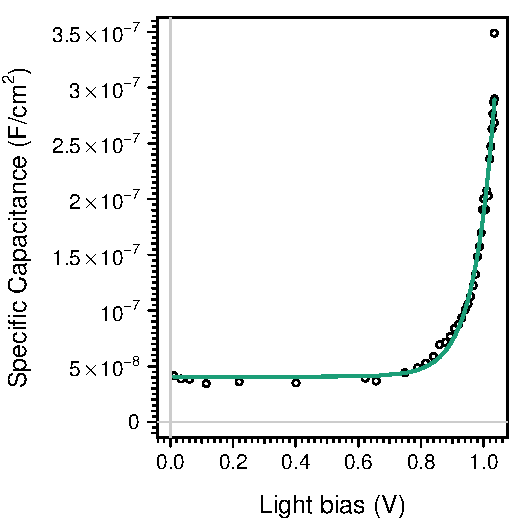
\includegraphics[width=1\textwidth]{cap_voltage_dependence/TAE-1_ig94-1559-1/DC-capacitance-TAE-1_ig94-1559-1.pdf}
		\subcaption{Perovskite solar cell.}\label{fig:cap_voltage_dependence_tae1}
	\end{subfigure}
	\mycaption[Capacitance dependence on applied voltage.]{In (a) the capacitance of a commercial capacitor is reported, it was measured using \acr{ce} with applied voltage bias instead of the classical light bias used for solar cells. The capacitance is obtained as the extracted charge over the applied voltage prior to short circuiting. In (b) the typical capacitance versus voltage profile of a \gls{fto}/\dTiOtwo/\mpTiOtwo/\acr{csfamapbibr}/\tae1/Au device is shown. In this case the indicated voltage is originated by various illumination intensities at open circuit prior to short circuiting.}\label{fig:cap_voltage_dependence}
\end{figure}

\section{Interpretation of Transient PhotoVoltage Referenced to Differential Capacitance}\label{interpretation_tpvdc}


\section{Varying MAPI Thickness (Absorber Material Layer)}
\section{Varying PCBM-C70 Thickness (Electron Transport Material Layer)}
\section{Varying PEDOT:PSS Thickness (Hole Transport Material Layer)}
\section{Critical Assessment}